%%%%%%%%%%%%%%%%%%%%%%%%%%%%%%%%%%%%%%%%%
% Beamer Presentation
% LaTeX Template
% Version 1.0 (10/11/12)
%
% This template has been downloaded from:
% http://www.LaTeXTemplates.com
%
% License:
% CC BY-NC-SA 3.0 (http://creativecommons.org/licenses/by-nc-sa/3.0/)
%
%%%%%%%%%%%%%%%%%%%%%%%%%%%%%%%%%%%%%%%%%

%----------------------------------------------------------------------------------------
%	PACKAGES AND THEMES
%----------------------------------------------------------------------------------------

\documentclass{beamer}

\mode<presentation> {

% The Beamer class comes with a number of default slide themes
% which change the colors and layouts of slides. Below this is a list
% of all the themes, uncomment each in turn to see what they look like.

%\usetheme{default}
%\usetheme{AnnArbor}
%\usetheme{Antibes}
%\usetheme{Bergen}
%\usetheme{Berkeley}
%\usetheme{Berlin}
%\usetheme{Boadilla}
%\usetheme{CambridgeUS}
%\usetheme{Copenhagen}
%\usetheme{Darmstadt}
%\usetheme{Dresden}
%\usetheme{Frankfurt}
%\usetheme{Goettingen}
%\usetheme{Hannover}
%\usetheme{Ilmenau}
%\usetheme{JuanLesPins}
%\usetheme{Luebeck}
\usetheme{Madrid}
%\usetheme{Malmoe}
%\usetheme{Marburg}
%\usetheme{Montpellier}
%\usetheme{PaloAlto}
%\usetheme{Pittsburgh}
%\usetheme{Rochester}
%\usetheme{Singapore}
%\usetheme{Szeged}
%\usetheme{Warsaw}

% As well as themes, the Beamer class has a number of color themes
% for any slide theme. Uncomment each of these in turn to see how it
% changes the colors of your current slide theme.

%\usecolortheme{albatross}
%\usecolortheme{beaver}
%\usecolortheme{beetle}
%\usecolortheme{crane}
%\usecolortheme{dolphin}
%\usecolortheme{dove}
%\usecolortheme{fly}
%\usecolortheme{lily}
%\usecolortheme{orchid}
%\usecolortheme{rose}
%\usecolortheme{seagull}
%\usecolortheme{seahorse}
%\usecolortheme{whale}
%\usecolortheme{wolverine}

%\setbeamertemplate{footline} % To remove the footer line in all slides uncomment this line
%\setbeamertemplate{footline}[page number] % To replace the footer line in all slides with a simple slide count uncomment this line

%\setbeamertemplate{navigation symbols}{} % To remove the navigation symbols from the bottom of all slides uncomment this line
}

\usepackage{graphicx} % Allows including images
\usepackage{bm}
\usepackage{booktabs} % Allows the use of \toprule, \midrule and \bottomrule in tables
\usepackage{color}
\usepackage{tikz}
\usepackage{amsmath}
\usepackage{framed}

\usetikzlibrary{topaths,calc}

\AtBeginSection[]{
  \begin{frame}
  \vfill
  \centering
  \begin{beamercolorbox}[sep=8pt,center,shadow=true,rounded=true]{title}
    \usebeamerfont{title}\insertsectionhead\par%
  \end{beamercolorbox}
  \vfill
  \end{frame}
}
%----------------------------------------------------------------------------------------
%	TITLE PAGE
%----------------------------------------------------------------------------------------
\title[Short title]{Knowledge Compilation und \#SAT}

\author{Narek Bojikian} % Your name
\institute[Hu-Berlin] % Your institution as it will appear on the bottom of every slide, may be shorthand to save space
{
Humboldt University of Berlin\\ % Your institution for the title page
}
\date{08.01.2019} % Date, can be changed to a custom date

\begin{document}

\begin{frame}
\titlepage % Print the title page as the first slide
\end{frame}

\begin{frame}[t]{Definitions}
\begin{itemize}
\uncover<1->{\item The SAT Problem (\textbf{SAT}).}
\uncover<2->{\item Counting SAT Problem (\textbf{\#SAT}).}


\uncover<6->{\item Negation Normal Form (\textbf{NNF}).}
\uncover<7->{\item Conjunctive Normal Form (\textbf{CNF}).}
\uncover<8->{\item Decomposable Negation Normal Form (\textbf{DNNF}).}
\uncover<9->{\item deterministic Decomposable Negation Normal Form (\textbf{d-DNNF}).}
\uncover<10->{\item decision Decomposable Negation Normal Form (\textbf{dec-DNNF}).}
\end{itemize}

\only<1>{
\begin{block}{SAT}
\begin{itemize}
\item[--] Given a Boolean formula $\varphi$ of $n$ variables.
\item[?] Find an assignment that satisfies $\varphi$.
\end{itemize}
\end{block}
}

\only<2>{
\begin{block}{\#SAT}
\begin{itemize}
\item[--] Given a Boolean formula $\varphi$ of $n$ variables.
\item[?] How many assignments in $2^{\mathrm{Var}(\varphi)}$ satisfy $\varphi$?
\end{itemize}
\end{block}
}

\only<3-4>{
\begin{block}{Notation}
Let $\mathrm{SAT}(\chi) \subseteq 2^{\mathrm{VAR}(\chi)}$ be the set of all satisfying assignments of $\chi$
\vspace{-0.3cm}
$$\mathrm{SAT}(\chi) = \{\rho:\mathrm{VAR}(\chi) \rightarrow \{0, 1\} : \rho(\chi) = 1\}.$$
\vspace{-0.8cm}
\uncover<4->{$$\text{SAT: Is } \mathrm{SAT}(\varphi) = \emptyset.
\qquad \qquad \qquad
\text{\#SAT: Find } |\mathrm{SAT}(\varphi)|.$$}
\vspace{-0.6cm}
\end{block}
}

\only<5>{
\begin{block}{Example}
$$\varphi = X_1 \land (X_2 \lor \lnot X_3)$$
Clearly, \#SAT($\varphi$) = 3.
\end{block}
}

\only<6>{
\begin{block}{Negation Normal Form}
A Boolean formula $\varphi$ is in NNF form, if it contains only disjunctions and conjunctions over a set of positive and(or) negative literals.

\textbf{Example.} $\varphi = X_1 \lor \lnot X_2$.
\end{block}
}

\only<7>{
\begin{block}{Conjunctive Normal Form}
A Boolean formula $\varphi$ is in CNF, if it is a conjunction of one or more clauses, where each clauses is a disjunction of one or more literals. Note that each CNF formula is an NNF formula as well.
\end{block}
}

\only<8>{
\begin{block}{Decomposable Negation Normal Form}
A Boolean formula $\varphi$ is in DNNF, if it is in NNF and for each conjunction subformula $phi' := \psi_1 \land \psi_2$ we have $\mathrm{VAR}(\psi_1) \cap \mathrm{VAR}(\psi_2) = \emptyset$.
\end{block}
}

\only<9>{
\begin{block}{deterministic Decomposable Negation Normal Form}
A Boolean formula $\varphi$ is in d-DNNF, if it is in DNNF and for each disjunction subformula  $\varphi' = \psi_1 \lor \psi_2$ we have $\mathrm{SAT}(\psi_1) \cap \mathrm{SAT}(\psi_2) = \emptyset$.
\end{block}
}

\only<10->{
\begin{block}{decision Decomposable Negation Normal Form}
A Boolean formula $\varphi$ is in dec-DNNF, if it is in DNNF and each disjunction subformula  $\varphi'$ is of the form $\varphi' = (X \land \psi_1) \lor (\lnot X \land \psi_2)$ for some variable $X \in \mathrm{VAR}(\varphi)$.

\uncover<11>{\textbf{Note.} Each dec-DNNF is a d-DNNF.}
\end{block}
}
\end{frame}

\begin{frame}[t]{Assignments}
	\begin{itemize}[<+->]
		\item Given a CNF Formula $\varphi$, an \textbf{assignment} for $C$ is a function $\tau : \mathrm{VAR}(C) \rightarrow \{0, 1\}$.
		\item For $V' \subseteq \mathrm{VAR}(C)$, we define the \textbf{partial assignment} $\tau_{|V'} : V' \rightarrow \{0, 1\}$ as $\tau$ restricted to the variables in $V'$.
		\item A partial assignment $\tau_{|V'}$ satisfies a CNF-formula $\varphi$ ($\tau_{|V'} \models \varphi$), if for each clause $C \in \varphi$ there is a variable $v \in \mathrm{VAR}(C) \cap V'$ such that $\tau_{|V'}(v) = 1$ if and only if $v$ appears in $C$ as a positive literal.

	\end{itemize}
	\uncover<4>{
	\begin{block}{Example}
		$$\varphi := (v_1 \lor \lnot v_2 \lor v_3) \land (v_1 lor v_2) \land (\lnot v2 \lor \lnot v_3)$$
		For $V' = \{v_1, v_2\}, \tau_{|V'}(v_1) = 1, \tau_{|v'}(v_2) = 0$,
		the partial assignment $\tau_{|V'}$ satisfies $\varphi$.
	\end{block}
	}
\end{frame}

\begin{frame}[t]{Structuredness of a formula}
	\begin{itemize}[<+->]
		\item Let $\varphi$ be a DNNF formula and let $V := \mathrm{VAR}(\varphi)$.
		\item A \textbf{$\mathbf{v}$Tree} $T$ is a binary tree where the leaves of the tree has a one-to-one correspondence to the variables of $\varphi$.
		\item The formula $\varphi$ respects $T$ if and only if for each subformula of  $\varphi$ of the form $\varphi' := \psi_1 \land \psi_2$, there is a vertex $v \in V(T)$ with two children $v_1, v_2$, where $\mathrm{VAR}(\psi_1)\subseteq V(T_{v_1})$ and $\mathrm{VAR}(\psi_2) \subseteq V(T_{v_2})$, where $T_v$ is the subtree of $T$ rooted at $v$. We say $\varphi'$ respects $v$ in this case.
		\item A formula $\varphi$ is structured, if there is a $v$tree $T$ over the vertices of $\varphi$, such that $\varphi$ respects $T$.
	\end{itemize}

	\uncover<3->{
	\begin{minipage}{.49\linewidth}
		$$(x\land(y\lor z)) \lor (z \textcolor{red}{\bm{\land}} \lnot x)$$
	\end{minipage}
	\hfill
	\begin{minipage}{.49\linewidth}
		\centering
		
\includegraphics[width=.6\linewidth]{figures/vtree.eps}
	\end{minipage}
	}
\end{frame}

\begin{frame}[t]{Hypergraphs and $\beta$-acyclic graphs}
	\begin{minipage}{.59\linewidth}
	\begin{itemize}
		\item Hypergraph $\mathcal{G}$.
			\begin{itemize}
				\item A set of vertices $V(\mathcal{G})$.
				\item Edges $E(\mathcal{G})$, defined as 
				\item[] subsets over $V(\mathcal{G})$.
			\end{itemize}

		\uncover<2->{\item Different ways to translate
		\item[] \hspace{1cm} acycli8ity to  hypergraphs.}

		\uncover<3->{\item $\beta$-acyclic hypergraphs.}
			\begin{itemize}
				\uncover<4->{\item Defined on the edges.}
				\uncover<5->{\item Let $\rho := v_1, \dots v_n$ be an
				\item[] \hspace{1cm}enumeration of the vertices.}
				\uncover<6->{\item $\rho$ is a $\beta$-elimination, if for all}
				\uncover<7->{\item[] \hspace{1cm}$e_1, e_2 \in E(\mathcal{G})$ and $v_i \in e_1 \cap e_2$,
				\item[]\hspace{1cm}$e_{1|\geq i} \subseteq e_2$ or $e_{2|\geq i} \subseteq e_1$.}
				\uncover<8->{\item A hypergraph is $\beta$-acyclic,
				\item[] \hspace{1cm} if it admits a $\beta$-elimination.}

			\end{itemize}
	\end{itemize}
\end{minipage}
\begin{minipage}{.39\linewidth}
\centering
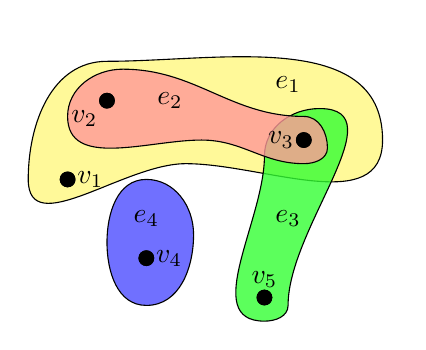
\begin{tikzpicture}
    \node (v1) at (1,2) {};
    \node (v2) at (1.5,3) {};
    \node (v3) at (4,2.5) {};
    \node (v4) at (2,1) {};
    \node (v5) at (3.5,0.5) {};

    \begin{scope}[fill opacity=0.8]
    \filldraw[fill=yellow!50] ($(v1)+(-0.5,0)$) 
        to[out=90,in=180] ($(v2) + (0,0.5)$) 
        to[out=0,in=90] ($(v3) + (1,0)$)
        to[out=270,in=0] ($(v2) + (1,-0.8)$)
        to[out=180,in=270] ($(v1)+(-0.5,0)$);
    \filldraw[fill=blue!70] ($(v4)+(-0.5,0.2)$)
        to[out=90,in=180] ($(v4)+(0,1)$)
        to[out=0,in=90] ($(v4)+(0.6,0.3)$)
        to[out=270,in=0] ($(v4)+(0,-0.6)$)
        to[out=180,in=270] ($(v4)+(-0.5,0.2)$);

    \filldraw[fill=green!80] ($(v3)+(-0.5,-0.2)$) 
        to[out=90,in=180] ($(v3) + (0.2,0.4)$) 
        to[out=0,in=90] ($(v5) + (0.3,-0.1)$)
        to[out=270,in=0] ($(v5) + (0,-0.3)$)
        to[out=180,in=270] ($(v3)+(-0.5,-0.2)$);

    \filldraw[fill=red!40] ($(v2)+(-0.5,-0.2)$) 
        to[out=90,in=180] ($(v2) + (0.2,0.4)$) 
        to[out=0,in=180] ($(v3) + (0,0.3)$)
        to[out=0,in=90] ($(v3) + (0.3,-0.1)$)
        to[out=270,in=0] ($(v3) + (0,-0.3)$)
        to[out=180,in=0] ($(v3) + (-1.3,0)$)
        to[out=180,in=270] ($(v2)+(-0.5,-0.2)$);
    \end{scope}

    \foreach \v in {1,2,...,5} {
        \fill (v\v) circle (0.1);
    }

    \fill (v1) circle (0.1) node [right] {$v_1$};
    \fill (v2) circle (0.1) node [below left] {$v_2$};
    \fill (v3) circle (0.1) node [left] {$v_3$};
    \fill (v4) circle (0.1) node [right] {$v_4$};
    \fill (v5) circle (0.1) node [above] {$v_5$};

    \node at (3.8,3.2) {$e_1$};
    \node at (2.3,3) {$e_2$};
    \node at (3.8,1.5) {$e_3$};
    \node at (2, 1.5) {$e_4$};
\end{tikzpicture}

\end{minipage}
\footnotetext[1]{$e_{|\geq i} := e \cap \{v_i, \dots v_n\}$.}
\end{frame}

\begin{frame}[t]{Incidence graphs and structure of formulas}
	\begin{itemize}
		\item The \textbf{incidence graph} of $\mathcal{G}$ is a 
		\item[] \hspace{1cm}bipartite graph $(V(\mathcal{G}) \cup E(\mathcal{G}), E)$
		\item[] \hspace{1cm},where $\{v, e\} \in E$ iff $v \in e$.
			\vspace{.5cm}
		\uncover<2->{\item Hypergraph of a CNF-Formula.}
		\uncover<3->{\item The incidence graph of a CNF-Formula is
		\item[] \hspace {1cm} the incidence graph of its hyper graph.}
		\uncover<4->{\item A CNF-Formula is $\beta$-acyclic if its hypergraph is.}
	\end{itemize}

\end{frame}
	


\section{Theoretical upper-bound on the practical method}
\begin{frame}[t]{Lemmas on $\beta$-acyclic graphs}
	\begin{itemize}[<+->]
	\item Let $\mathcal{H}$ be a $\beta$-acyclic graph and $v_1, \dots v_n$ a $\beta$-elimination.
		\item For two edge $e, f \in \mathcal{H}$, $e < f$, if and only if $\max\{e \Delta f\}\in f$
		\item {\color{blue}$\mathcal{H}^x_e$} denotes the subgraph of $\mathcal{H}$, that contain the edges $f$, such that there is a walk from $f$ to $e$ that goes only through edges smaller than $e$ and vertices smaller than (or equal to) $x$.
	\end{itemize}
	\begin{figure}[htpb]
		\centering
		\resizebox{.6\columnwidth}{!}{
		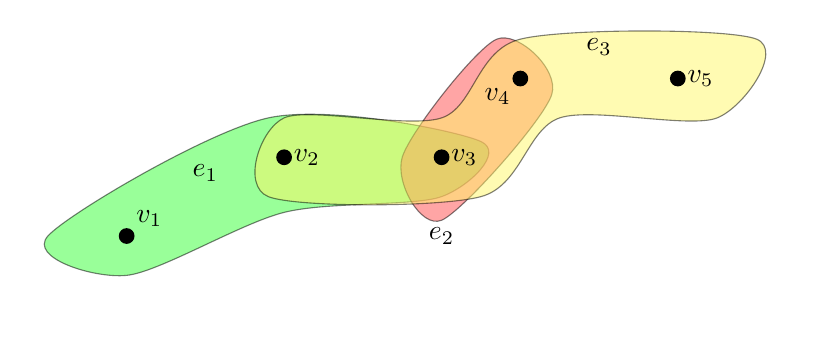
\begin{tikzpicture}
	\node (u) at (0, 0) {};
	\node (v) at (3, 3) {};

	\node (v1) at (1, 1) {};
	\node (v2) at (3, 2) {};
	\node (v3) at (5, 2) {};
	\node (v4) at (6, 3) {};
	\node (v5) at (8, 3) {};
	\begin{scope}[opacity=.5]
	\draw [draw=black, fill=green!80] plot [smooth cycle] coordinates {
			($(v1) + (0,-.5)$) ($(v1) + (-1,0)$) ($(v2) + (-.2,.5)$)
			($(v3) + (.5, .2)$) ($(v3) + (0, -.5)$) ($(v2) + (0, -.7)$)};

	\draw [draw=black, fill=red!70] plot [smooth cycle] coordinates {
			($(v3) + (0,-.8)$) ($(v3) + (-.5,0)$)
			($(v4) + (-.3, .5)$) ($(v4) + (.4, -.2)$)
		};
	\draw [draw=black, fill=yellow!60] plot [smooth cycle] coordinates {
			($(v2) + (0,.5)$) ($(v3) + (0,.5)$) ($(v4) + (0,.5)$)
			($(v5) + (1,.5)$) ($(v5) + (.5,-.5)$) ($(v4) + (.5,-.5)$) 
			($(v3) + (.5,-.5)$) ($(v2) + (-.2,-.5)$) 
		};
	\end{scope}

	\fill (v1) circle (0.1) node[above right] {$v_1$};
	\fill (v2) circle (0.1) node[right] {$v_2$};
	\fill (v3) circle (0.1) node[right] {$v_3$};
	\fill (v4) circle (0.1) node[below left] {$v_4$};
	\fill (v5) circle (0.1) node[right] {$v_5$};

	\node at (2,1.8) {$e_1$};
	\node at (5,1) {$e_2$};
	\node at (7,3.4) {$e_3$};
\end{tikzpicture}

		}
		\uncover<4->{\caption{Note that $e_2 \notin H^{v_2}_{e_3}$ meanwhile $e_2 \in H^{v_3}_{e_3}$}}
		\label{fig:name}
	\end{figure}
\end{frame}
\begin{frame}[t]{Lemmas on $\beta$-acyclic graphs}
	\begin{block}{Lemma (lemma 2)}
		For $x,y \in V(\mathcal{H}), x \leq y$ and for $e, f \in \mathcal{H}, e \leq f$,
			$$\text{if } V(\mathcal{H}^x_e)\cap V(\mathcal{H}^y_f)\cap V_{\leq x} \neq \emptyset,
			\text{ then } \mathcal{H}^x_e \subseteq \mathcal{H}^y_f.$$
			In particular, for all $y \in V(\mathcal{H})$,
		$$\text{if } e \in \mathcal{H}^y_f, \text{ then } \mathcal{H}^y_e \subseteq \mathcal{H}^y_f$$
	\end{block}
	\uncover<2->{
	Proof sketch. For $g \in \mathcal{H}^x_e$, there is a path from $g$ to $e$ using edges smaller than $e$ and vertices smaller than $x$.
	
	There is also a path from $e$ to $f$. Concatenate both paths to get a path from $g$ to $f$.
	}
\end{frame}

\begin{frame}[t]{Lemmas on $\beta$-acyclic graphs}
	\begin{block}{Lemma (lemma 4)}
		For $e, f \in \mathcal{H}, e\leq f$, If there exists a vertex $x \in V(\mathcal{H})$, such that $x \in e \cap f$, then $e \cap V_{\geq x} \subseteq f$.
	\end{block}
	\uncover<2->{
	Proof sketch. If $y \in e \setminus f$ such that $y > x$, then $\mathcal{H}$ is not $\beta$-acyclic.
	}
\end{frame}

\begin{frame}[t]{Lemmas on $\beta$-acyclic graphs}
	A path $(e_1, x_1, \dots e_{n+1})$ is called decreasing, if $e_i > e_{i+1}$ and $x_i > x_{i+1}$ for all $i$.
	\begin{block}{Lemma (lemma 5)}
		For $x \in V(\mathcal{H}), e \in \mathcal{H}$ and $f \in \mathcal{H}^x_e$, there exists a decreasing path from $e$ to $f$ going through vertices smaller than $x$.
	\end{block}
	\uncover<2->{Proof sketch. Any shortest path from $e$ to $f$ is decreasing. A path exists by definition.}
\end{frame}

\begin{frame}[t]{Lemmas on $\beta$-acyclic graphs}
	\begin{block}{Theorem (theorem 3)}
		For every $x \in V(\mathcal{H})$ and $e \in \mathcal{H}, V(\mathcal{H}^x_e) \cap V_{\geq x} \subseteq e$
	\end{block}

	\begin{center}
		\resizebox{.5\columnwidth}{!}{
		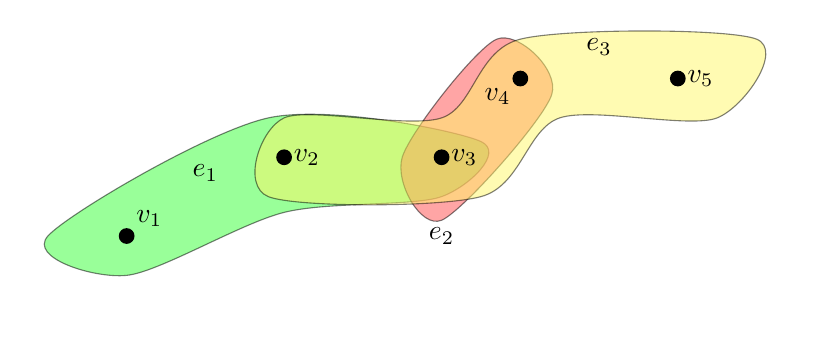
\begin{tikzpicture}
	\node (u) at (0, 0) {};
	\node (v) at (3, 3) {};

	\node (v1) at (1, 1) {};
	\node (v2) at (3, 2) {};
	\node (v3) at (5, 2) {};
	\node (v4) at (6, 3) {};
	\node (v5) at (8, 3) {};
	\begin{scope}[opacity=.5]
	\draw [draw=black, fill=green!80] plot [smooth cycle] coordinates {
			($(v1) + (0,-.5)$) ($(v1) + (-1,0)$) ($(v2) + (-.2,.5)$)
			($(v3) + (.5, .2)$) ($(v3) + (0, -.5)$) ($(v2) + (0, -.7)$)};

	\draw [draw=black, fill=red!70] plot [smooth cycle] coordinates {
			($(v3) + (0,-.8)$) ($(v3) + (-.5,0)$)
			($(v4) + (-.3, .5)$) ($(v4) + (.4, -.2)$)
		};
	\draw [draw=black, fill=yellow!60] plot [smooth cycle] coordinates {
			($(v2) + (0,.5)$) ($(v3) + (0,.5)$) ($(v4) + (0,.5)$)
			($(v5) + (1,.5)$) ($(v5) + (.5,-.5)$) ($(v4) + (.5,-.5)$) 
			($(v3) + (.5,-.5)$) ($(v2) + (-.2,-.5)$) 
		};
	\end{scope}

	\fill (v1) circle (0.1) node[above right] {$v_1$};
	\fill (v2) circle (0.1) node[right] {$v_2$};
	\fill (v3) circle (0.1) node[right] {$v_3$};
	\fill (v4) circle (0.1) node[below left] {$v_4$};
	\fill (v5) circle (0.1) node[right] {$v_5$};

	\node at (2,1.8) {$e_1$};
	\node at (5,1) {$e_2$};
	\node at (7,3.4) {$e_3$};
\end{tikzpicture}

		}
	\end{center}
	\uncover<2->{Proof sketch. Prove that all edges of a decreasing path are subsets of the first edge by induction over the length of the path.}

	\uncover<3->{Intuitively, this allows us to use dynamic programming, since all variables in $\mathcal{H}^x_e$ not contained in $e$ are smaller than $x$.}

\end{frame}


\begin{frame}[t]{Solving \#SAT in $\beta$-acyclic graphs}
	\begin{itemize}[<+->]
	\item The hypergraph of a CNF-formula:
	\item[]\hspace{1cm}Variables of each clause correspond to an edge.
	\item[]\hspace{1cm}Two clauses might correspond to the same edge.
	\item A $\beta$-acyclic CNF-formula F is given.
	\item Let $\mathcal{H}$ be the hypergraph of $F$.
	\item Let $v_1, \dots v_n$ be an elimination order in $\mathcal{H}$.
	\item Let {\color{blue}$F^x_e$} be the subformula of $F$ that corresponds to $\mathcal{H}^x_e$,

	\hspace{1cm}i.e. $C \in F^x_e$, if $\mathrm{VAR}(C) \in \mathcal{H}^x_e$.
	\item For a clause $C$, the partial assignment {\color{blue}$\tau_C$} is defined over $\mathrm{VAR}(C)$ as the only assignment that does not satisfy $C$,
	\item[]\hspace{1cm}i.e. for $x \in C$, $\tau_C(x) = 1$ if and only if $x$ appears as a negative literal in $C$.
	\item We define ${\color{blue}\tau^x_C} := \tau_{C|\geq x}$,
	\item[]\hspace{1cm}{\color{blue} $F[\tau^x_C]$} results from $F$ by removing all variables greater than $x$ from each clause.
	\end{itemize}
\end{frame}
\begin{frame}[t]{Solving \#SAT in $\beta$-acyclic graphs}
	\begin{block}{Lemma (lemma 6)}
		Let $x \neq x_1 \in \mathrm{VAR}(F)$ and let $y$ be the predecessor of $x$ for $<$. Let $e \in \mathcal{H}$ and $\tau : (e \cap V_{\geq x}) \rightarrow \{0, 1\}$. Then either $F^x_e[\tau] \equiv 1$ or there exists $U \subseteq \mathcal{H}^x_e$ such that 
		$$ F^x_e[\tau] \equiv \bigwedge\limits_{g \in U} F^y_g[\tau^y_{C_g}],$$
		where $C_g$ is some clause in $F^x_e$ such that $\mathrm{VAR}(C_g) = g$.
		
		Moreover, all and-gates are decomposable and $U$ can be computed in polynomial time.
	\end{block}
\end{frame}
\begin{frame}[t]{Solving \#SAT in $\beta$-acyclic graphs}
	\vspace{-1cm}
	\begin{center}
		$$ F^x_e[\tau] \equiv \bigwedge\limits_{g \in U} F^y_g[\tau^y_{C_g}],$$
	\end{center}
	Proof sketch.
	\begin{itemize}[<+->]
		\item Let $A$ be the set edges $g$, where $\tau \not \models C_g$ for some {\color{gray} \textit{corresponding}} $C_g$.
		\item For each clause $C$ such that $\mathrm{VAR}(C) \notin A$ we have $\tau \models C$.
		\item Choose $U$ as the set of "maximal" edges $g \in A$,
		\item For each $f \in A$, there is $g \in U$ such that $f \in \mathcal{H}^y_g$.
		\item[]\hspace{1cm}i.e. $g \not \subseteq \mathcal{H}^y_f$ for all $f \in A$, $f \neq g$.
		\item $U$ can be computed in polynomial time.
		\item The edges in $U$ are pairwise disjoint. Hence, the and-gate is  decomposable. 
	\end{itemize}
\end{frame}

\begin{frame}[t]{Solving \#SAT in $\beta$-acyclic graphs}
	\begin{block}{Corollary (corollary 7)}
		Let $x \neq x_1 \in \mathrm{VAR}(F)$ and let $y$ be the predecessor of $x$ for $<$. For every $C \in \mathcal{H}$, there exist $U_0, U_1 \subseteq \mathcal{H}^x_{\mathrm{VAR}(C)}$ such that
		$$F^x_{\mathrm{VAR}(C)}[\tau^x_C] \equiv 
		( x \land \bigwedge\limits_{g \in U_1} F^y_g[\tau^y_{C_g}]) \lor
		( \lnot x \land \bigwedge\limits_{g \in U_2} F^y_g[\tau^y_{C_g}]).
		$$
		Moreover, all conjunctions are decomposable and $U_0, U_1$ can be computed in polynomial time.
	\end{block}

	\pause
	Proof sketch. Let $\tau_1 := \tau^x_C \cup \{x \mapsto 1\}$ and $\tau_0 := \tau^x_C \cup \{x \mapsto 0\}$.
	$$F^x_{\mathrm{VAR}(C)}[\tau^x_C] = (x \land F^x_{\mathrm{VAR}(C)}[\tau_1]) \lor (\lnot x \land F^x_{\mathrm{VAR}(C)}[\tau_0])$$	
		Apply lemma 6 on each of the terms.
\end{frame}

\begin{frame}[t]{Solving \#SAT in $\beta$-acyclic graphs}
	\begin{block}{Theorem (theorem 8)}
		Let $F$ be a $\beta$-acyclic CNF-formula. One can construct in polynomial time in $\mathrm{size}(F)$ a dec-DNNF $D$ of size $O(\mathrm(size(F))$ and fanin at most $|\mathcal{H}|$ computing F.
	\end{block}
	\pause
	Proof sketch.
	Let $D_i$ be a dec-DNNF of fanin $|\mathcal{H}|$ at most such that for each $e \in \mathcal{H}, C \in F$ such that $\mathrm{VAR}(C) = e$ and $j \leq i$, there exists a gate in $D_i$ computing $F^{x_j}_e[\tau^{x_j}_c]$.
	\pause
	\begin{itemize}[<+->]
		\item Construct $D_i$ inductively over $i$.
		\item For an edge $e$, distinguish the cases whether $v_i \in e$ or not.
		\item For $i=1$,
		\item[]\hspace{1cm}$v_1 \notin e$: $F^{v_1}_e[\tau_C] = 0$.
		\item[]\hspace{1cm}$v_1 \in e$: $F^{v_1}_e \in \{1, v_1, \lnot v_1\}$.
	\end{itemize}
\end{frame}
\begin{frame}[t]{Proof sketch of theorem 8}
	\begin{itemize}[<+->]
		\item If $v_{i+1} \notin e$, then $F^{x_{i+1}}_e = F^{x_i}_e$.

		\item If $v_{i+1} \in e$, then by corollary 7 we can compute $F^{x_{i+1}}_e$ by adding a decision gate and (two) fanin at most $\mathcal{H}$ decomposable and-gates.
		
		\item[]\hspace{1cm}For each other terms from corollary 7 there is already a gate in $D_i$ that computes this term by induction hypothesis. 
		\item For $e = \max\mathcal{H}$ and a clause $C$ such that $\mathrm{VAR}(C) = e$, we have $\mathcal{H}^{v_n}_e = \mathcal{H}$ and $\tau^{x_n}_{\mathrm{VAR}(C)} = \emptyset$, hence there is a gate in $D_n$ computing $F^{x_n}_e[\tau_C] = F$.
		\item We add at most 7 gates per edges per vertex.
	\end{itemize}

\end{frame}

\begin{frame}[t]{Example}
	\begin{center}
		\resizebox{.45\columnwidth}{!}{
		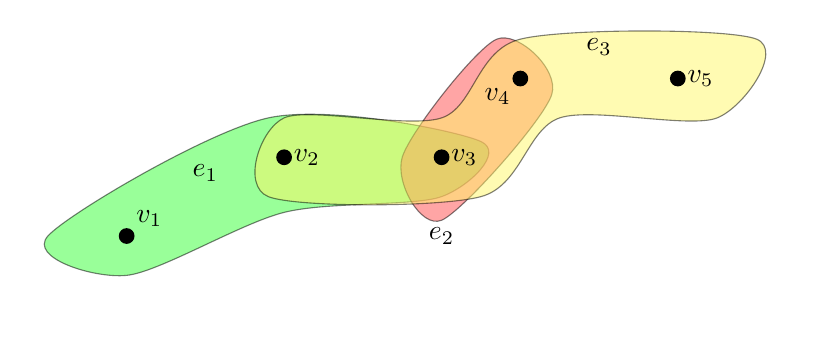
\begin{tikzpicture}
	\node (u) at (0, 0) {};
	\node (v) at (3, 3) {};

	\node (v1) at (1, 1) {};
	\node (v2) at (3, 2) {};
	\node (v3) at (5, 2) {};
	\node (v4) at (6, 3) {};
	\node (v5) at (8, 3) {};
	\begin{scope}[opacity=.5]
	\draw [draw=black, fill=green!80] plot [smooth cycle] coordinates {
			($(v1) + (0,-.5)$) ($(v1) + (-1,0)$) ($(v2) + (-.2,.5)$)
			($(v3) + (.5, .2)$) ($(v3) + (0, -.5)$) ($(v2) + (0, -.7)$)};

	\draw [draw=black, fill=red!70] plot [smooth cycle] coordinates {
			($(v3) + (0,-.8)$) ($(v3) + (-.5,0)$)
			($(v4) + (-.3, .5)$) ($(v4) + (.4, -.2)$)
		};
	\draw [draw=black, fill=yellow!60] plot [smooth cycle] coordinates {
			($(v2) + (0,.5)$) ($(v3) + (0,.5)$) ($(v4) + (0,.5)$)
			($(v5) + (1,.5)$) ($(v5) + (.5,-.5)$) ($(v4) + (.5,-.5)$) 
			($(v3) + (.5,-.5)$) ($(v2) + (-.2,-.5)$) 
		};
	\end{scope}

	\fill (v1) circle (0.1) node[above right] {$v_1$};
	\fill (v2) circle (0.1) node[right] {$v_2$};
	\fill (v3) circle (0.1) node[right] {$v_3$};
	\fill (v4) circle (0.1) node[below left] {$v_4$};
	\fill (v5) circle (0.1) node[right] {$v_5$};

	\node at (2,1.8) {$e_1$};
	\node at (5,1) {$e_2$};
	\node at (7,3.4) {$e_3$};
\end{tikzpicture}

		}
		$$F = \{\{\overline{v_1}, v_2, v_3\}, \{\overline{v_3}, v_4\}, \{v_2, v_3, \overline{v_4}, \overline{v_5}\}\}$$
	\end{center}
	\vspace{1cm}\hspace{7cm}The rest on the blackboard..
\end{frame}
\begin{frame}[t]{concluding the practical method}
	\begin{itemize}[<+->]
		\item Exhaustive DPLL is a very-well used in practice method.
			\begin{itemize}
				\item Try to write $F$ as a decomposable conjunction. 
				\item[] \hspace{1cm}Solve independently on each and multiply the results.
				\item Choose a variable $x$.
				\item[] \hspace{1cm}Compute $\#F[x\mapsto 1] + \#F[x\mapsto 0]$.
			\end{itemize}
		\item The method makes use of cashing (choose what values to keep).
		\item Tries to find a good candidate for $x$.
		\item The previous dynamic programming is implicitly a run of DPLL. 
		\item The variables are chosen in e reversed $\beta$-elimination ordering. 
	\end{itemize}
	\uncover<10->{\begin{block}{conclusion}
		Exhaustive DPLL can yield efficient algorithms "theoretically", if we can find a good order to choose the variable (such an ordering must be computable in polynomial time) and a good method of cashing.
	\end{block}}
\end{frame}

\section{Hardness of the theoretical method}
\begin{frame}[t]{Structuredness of a formula}
	\begin{itemize}[<+->]
		\item Let $\varphi$ be a DNNF formula and let $V := \mathrm{VAR}(\varphi)$.
		\item A \textbf{$\mathbf{v}$Tree} $T$ is a binary tree where the leaves of the tree has a one-to-one correspondence to the variables of $\varphi$.
		\item The formula $\varphi$ respects $T$ if and only if for each subformula of  $\varphi$ of the form $\varphi' := \psi_1 \land \psi_2$, there is a vertex $v \in V(T)$ with two children $v_1, v_2$, where $\mathrm{VAR}(\psi_1)\subseteq V(T_{v_1})$ and $\mathrm{VAR}(\psi_2) \subseteq V(T_{v_2})$, where $T_v$ is the subtree of $T$ rooted at $v$. We say $\varphi'$ respects $v$ in this case.
		\item A formula $\varphi$ is structured, if there is a $v$tree $T$ over the vertices of $\varphi$, such that $\varphi$ respects $T$.
	\end{itemize}

	\uncover<3->{
	\begin{minipage}{.49\linewidth}
		$$(x\land(y\lor z)) \lor (z \textcolor{red}{\bm{\land}} \lnot x)$$
	\end{minipage}
	\hfill
	\begin{minipage}{.49\linewidth}
		\centering
		
\includegraphics[width=.6\linewidth]{figures/vtree.eps}
	\end{minipage}
	}
\end{frame}

\begin{frame}[t]{Incidence graphs and structure of formulas}
	\begin{itemize}
		\item The \textbf{incidence graph} of $\mathcal{H}$ is a 
		\item[] \hspace{1cm}bipartite graph $(V(\mathcal{H}) \cup E(\mathcal{H}), E)$
		\item[] \hspace{1cm},where $\{v, e\} \in E$ iff $v \in e$.
			\vspace{.5cm}
		\uncover<2->{\item Hypergraph of a CNF-Formula.}
		\uncover<3->{\item The incidence graph of a CNF-Formula is
		\item[] \hspace {1cm} the incidence graph of its hyper graph.}
		\uncover<4->{\item A CNF-Formula is $\beta$-acyclic if its hypergraph is.}

		\item {}[todo] MIM-width
		\item []example on the board.
	\end{itemize}

\end{frame}
\begin{frame}{Results on the structured d-DNNF}
\end{frame}

\end{document} 
